\part{Microservice Design - First Advice}


\begin{frame}{Questions Addressed in this Section}
So far we were concerned with writing \textit{one} microservice well. 
\vfill
Some additional key design topics for cloud-native applications are:  
\begin{itemize}
	\item How to split functionality into microservices?
    \item How do services communicate with each other?
    \item How to design microservices internally?
    \item What is the scaling model?
	\item How to set up your development organization?
    \item Where to find resources and design guidance?
\end{itemize}
\vfill
This section gives \textit{initial guidance} on how to start.
\end{frame}


\begin{frame}{Disclaimer}
\center{
    \huge
    \textbf{Disclaimer!}
    \large
    \vfill
    This section does not claim to really explain the relevant topics of design, architecture, team setup, process etc. \\
    \vfill
    The goal is just to give a rough idea and create awareness to the topic that you really need to work on in your project!
    \vfill
    \small
    Applies to new cloud-native applications, not to XSA.
}
\end{frame}


\begin{frame}[t]{Microservice Disasters}
\textbf{One example story on how NOT to do it:}
%\footnotesize
\begin{itemize}
    \item Broken down a monolith into \textbf{150} microservices
    \item > 100 developers, 18 months, everyone wrote 'their service'
    \item One architecture guideline: No data duplication!
    \item Other guideline: REST APIs (synchronous!) for everything, huge number of internal API calls, no hystrix used
    \item REST calls took on average 150 ms, target SLA 99.9\% ; \\
          200 calls needed to service one outside request; => 13\% SLA
    \item No continuous integration / - delivery / automation infrastructure
\end{itemize}
\vfill
For the full story, watch \colorlink{https://www.youtube.com/watch?v=gfh-VCTwMw8}{this video}.
\end{frame}


\begin{frame}{Introduction to Domain Driven Design}
\begin{block}{DDD is a \textbf{Design Method} }
\vspace{-3mm}
    \small
    \begin{itemize}
     \item invented by Eric Evans for large system development / - evolution, \\
           fits very well for cloud-native applications 
   	 \item leads to \textit{highly cohesive} and \textit{loosely coupled services}
	\end {itemize}
\vspace{-3mm}
\end{block}

\vfill
\textbf{DDD - \textit{Strategic Design} Level}
\begin{itemize}
    \item Concerned with finding the domains and subdomains of your application. 
    \begin{itemize}
        \item \textbf{Core Domain}: Your area of innovation/IP
        \item \textbf{Generic Domain}: Stuff that many apps need, e.g. user management
        \item \textbf{Supporting Domain}: In-between, specific to your case
    \end{itemize}
    \item Key: \textit{Focus DDD design efforts on the Core Domain!}
    \item Buy generic -, build core and supporting domain code.
\end{itemize}
\end{frame}


\begin{frame}{Context Maps}
A context map is useful to show the Domains / Bounded Contexts, their types and relationships. 
\vfill
\centerline{
    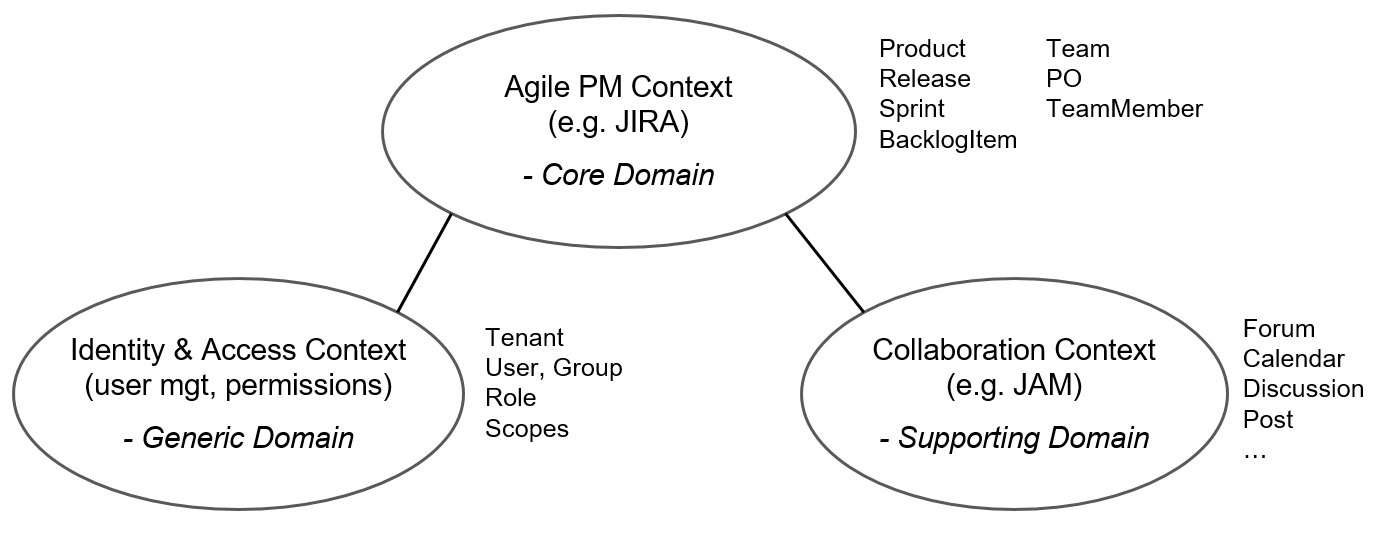
\includegraphics[height=0.5\textheight]{../MicroServiceDesign/images/ContextMapExample}
}
\end{frame}


\begin{frame}{Model Discovery and Bounded Contexts}
Identify core concepts in the domain by modeling key use cases. 
\begin{itemize}
    \item The same \textbf{term} usually means different things in different contexts. Model (and implement) them separately, i.e. with \textit{separate data}
    \item A \textbf{Bounded Context} is a domain scope where concepts and language are logically complete and consistent.
\end{itemize}
\vfill
\centerline{
    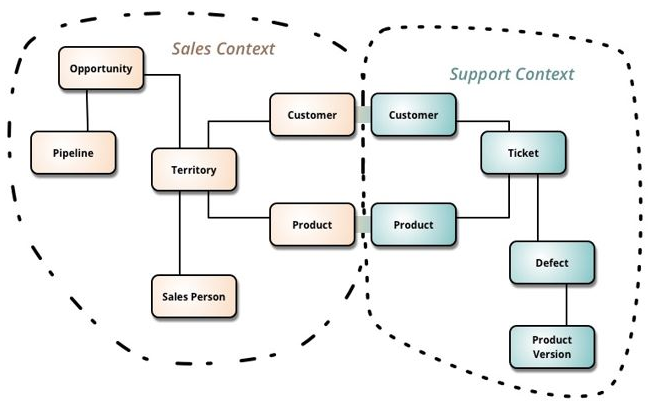
\includegraphics[height=0.5\textheight]{../MicroServiceDesign/images/MicroServiceDesign}
}
\end{frame}


\begin{frame}{Event Storming for Business Process Discovery}
\begin{columns}
\begin{column}{.4\textwidth}
\begin{block}{Event Storming}
    \vspace{-3mm}
    \small
    \begin{itemize}
	\item Outside-in domain modeling approach
        \item Often a moderated workshop with developers and domain experts
	\item \textbf{\textit{Focus on business process, not on data!}}
	\end {itemize}
    \vspace{-3mm}
\end{block}
\vspace{-3mm}
   \small
   \begin{itemize}
        \item Start with modeling process by relevant \textbf{business events}
        \item Identify needed data --> Identify domains and sub-domains
    \end{itemize}
    \vfill
\end{column}
\begin{column}{.58\textwidth}
    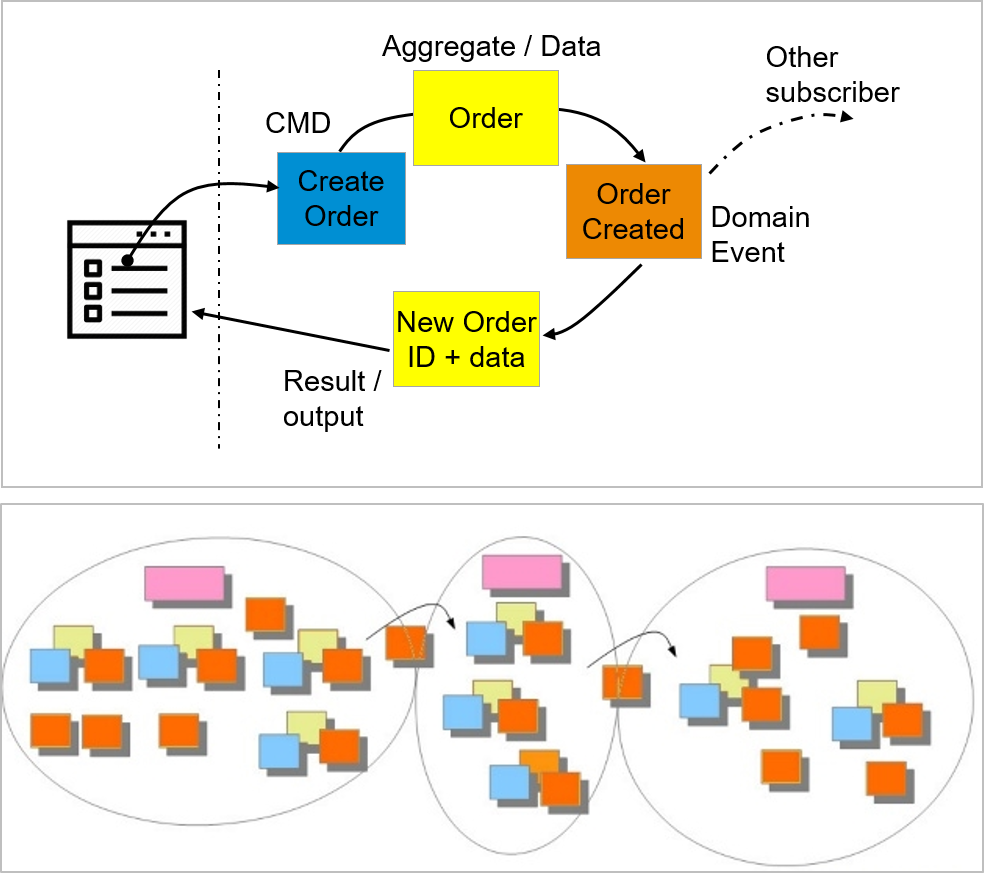
\includegraphics[height=60mm]{../MicroServiceDesign/images/EventStorming3}
\end{column}
\end{columns}
\end{frame}


\begin{frame}[t]{Key Elements of DDD Implementation Design}
\begin{itemize}
    \item \textbf{Entity}: Has identity and attributes (e.g. Customer, Order)
    \item \textbf{ValueObject (VO)}: Has NO identity (e.g. Address), favor VOs
    \item \textbf{Aggregate}: A few entities and VOs that have common lifetime, saved and loaded as one
    \item \textbf{Invariant}: Consistency rule that must be true, implemented at aggregate level, defines transaction boundary
    \item \textbf{DomainEvent}: Something relevant happened in system, used \textit{within and between} microservices for eventual consistency
    \item \textbf{Factories} create aggregates, \textbf{Repositories} manage persistence
\end{itemize}
\textbf{Good aggregate design is a key ingredient to scalability.}
\end{frame}


\begin{frame}[t]{Making the Right Architecture / Design Choices}
Remember the microservice architecture constraints:
\begin{itemize}
    \item Each MS has its own and separate data / DB
    \item No transaction across MSs; instead eventual consistency
    \item Calls between MSs are 10000x slower\footnote{REST call $\approx$ 10-20 ms; Java method call < 1$\mu$s} than within
    \item Must design for failure everywhere (hardware, software)
    \item Scale horizontally
    \item Build in resilience to reach > 99.99\%
\end{itemize}
\end{frame}



\begin{frame}[t]{Initial Design Guidelines}
\textbf{First: Know your domain! Then start with these guidelines:}
%\footnotesize
\begin{itemize}
    \item Start with a few microservices, one MS per Bounded Context. 
    \begin{itemize}
      \item Separate out smaller MSs only when needed for scalability.
    \end{itemize}
    \item A MS owns some data and replicates some data from others \\ 
    $\Rightarrow$ can answer most requests without synchr. calls to other MSs. 
    \item Use async. messages / events for updates between MSs.  
\end{itemize}
%\vspace{-2mm}
\center{
    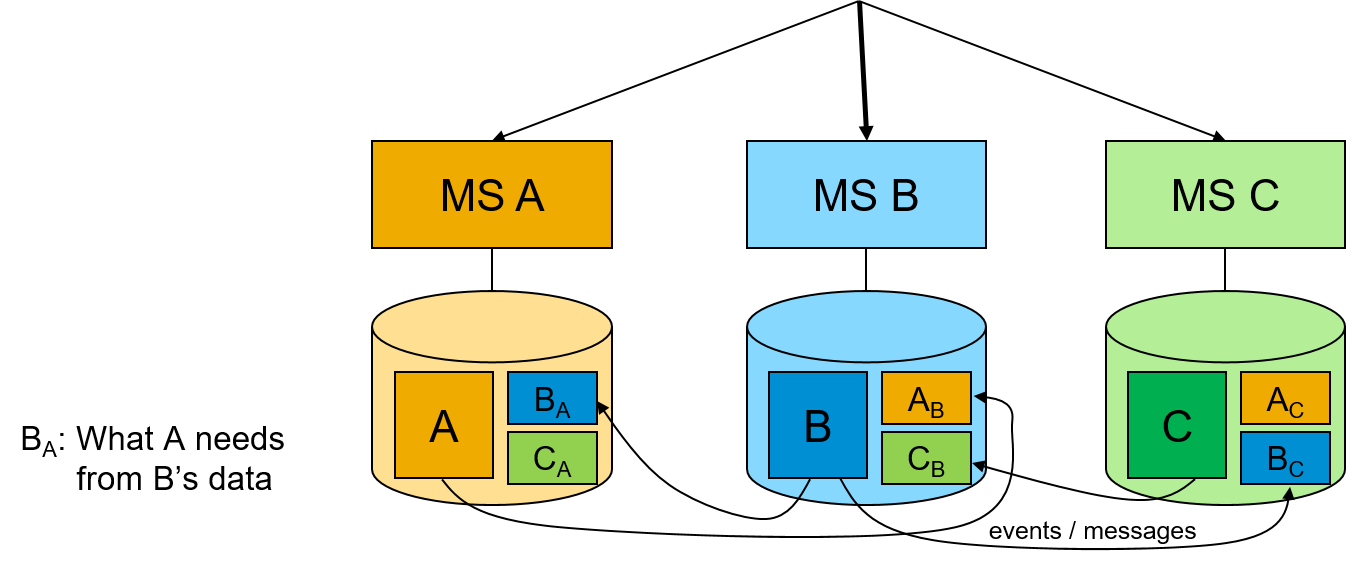
\includegraphics[height=33mm]{../MicroServiceDesign/images/3ServicesWithMsgs}
}
\end{frame}


\begin{frame}{High Level Guidance}
\begin{itemize}
    \item Managers and architects: Read "Building Microservices"
    \item Architects and devs: Read "Implementing Domain Driven Design"
    \item Go to an external DDD training \& apply it for your 'Core Domain' 
    \item Design with load and TCO in mind!
    \item Implement full test automation and Continuous Delivery
    \item Organize teams to own 1-2 Services each ('Conways Law')
\end{itemize}
\center{
    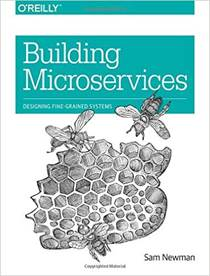
\includegraphics[height=24mm]{../MicroServiceArchitecture/images/buildingMicroservices}
    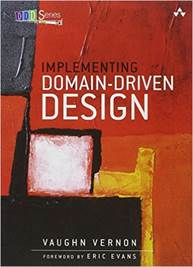
\includegraphics[height=24mm]{../MicroServiceArchitecture/images/implementingDomainDrivenDesign}
}
\end{frame}


\begin{frame}{Resources and Further Reading}
\begin{columns}
\begin{column}{.65\textwidth}
\textbf{References}
	\footnotesize
	\begin{itemize}
        \item \colorlink{https://jam4.sapjam.com/discussions/Ufud4ZPrq9hIxGwhlTg449}{DDD and Cloud Application Design Forum}
        \item \colorlink{https://elearn.domainlanguage.com/}{'DDD eLearning'} by Eric Evans
	\item \colorlink{https://jam4.sapjam.com/wiki/show/eBIJTH4EwfD15ymE2nv2pG}{Microservices Guidance Paper}\\
		 SAP CTO Circle Whitepapers (internal)
	\item \colorlink{https://jam4.sapjam.com/groups/w12lqZCV3pTdERnuIUMcBO/documents/hWzUxoEzpOHfaMcN5qbQ7K}{Domain Driven Design (internal)}
	\item \colorlink{https://jam4.sapjam.com/blogs/show/spPIuI94GYS4rtjCPWttrq}
				{Microservice Talk by Martin Fowler} at SAP
	\item \colorlink{https://jam4.sapjam.com/blogs/show/e47wfOsEwnYFyVtOWjb3nt?_lightbox=true}
				{Criteria for defining Microservices at SAP}  (Architecture Group)
	\item \colorlink{http://www.amazon.de/Building-Microservices-Sam-Newman/dp/1491950358/ref=sr_1_1}
				{Splitting the monolith} \\
				(Chapter 5 of 'Building Microservices')
	\item \colorlink{https://msdn.microsoft.com/en-us/library/dn568099.aspx}
				{Cloud Design Patterns (Microsoft)}
	\item \colorlink{https://dev.otto.de/2015/09/30/on-monoliths-and-microservices/}
				{Microservice Architecture of Otto.de}
	\end{itemize}
\end{column}
\begin{column}{.30\textwidth}
\footnotesize
\textbf{Recommended Reading}
	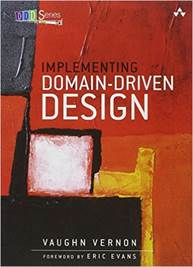
\includegraphics[height=22mm]{../MicroServiceArchitecture/images/implementingDomainDrivenDesign}
	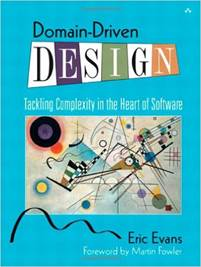
\includegraphics[height=22mm]{../MicroServiceArchitecture/images/domainDrivenDesign}
\end{column}
\end{columns}
\end{frame}
